\documentclass[../main.tex]{subfiles}
\begin{document}

\subsection{Prompt Templates}\label{clean_up:prompts}

The prompt templates for both players of Clean Up are given in Figure~\ref{fig:clean_up_prompt_templates}.

Intermittent messages sent by the Game Master to the players are given in Figure~\ref{fig:clean_up_intermittent_prompts}. Following a player's response, they are either penalized and reprompted (cf. Figure~\ref{fig:clean_up_format_error}, \ref{fig:clean_up_invalid_move}), or the turn is passed to the other player (Figure~\ref{fig:clean_up_new_turn}).

\begin{figure*}
  \centering
  \begin{prompt}
  I am your game master, and you are playing a collaborative game with the following grid as game board:\\
  
\includegraphics[height=120pt]{clean_up/example_grid.pdf}\\
* The upper edge displays x-coordinates increasing to the right, and the right edge y-coordinates increasing downward.\\
* The following objects are randomly placed on your grid: 'W', 'I', 'T', 'C', 'H'.\\
The other player sees a variation of the game board, where the objects are placed at different random locations. You cannot see the other player's board, and they cannot see yours.\\
\\
**Goal:**\\
Both players need to move the objects on their respective background so that identical objects end up at the same coordinates. You have to communicate with the other player to agree upon a common goal configuration.\\
\\
**Rules:**\\
* In each turn, you can send exactly one of the following two commands:\\
 1. \verb|`SAY: <MESSAGE>`|: to send a message (everything up until the next line break) to the other player. I will forward it to your partner.\\
2. \verb|`MOVE: <OBJECT>, (<X>, <Y>)`|: to move an object to a new position, where \verb|`<X>`| is the column and \verb|`<Y>`| is the row. I will inform you if your move was successful or not.\\
* If you don't stick to the format, or send several commands at once, I have to penalize you.\\
* If both players accumulate more than 12 penalties, you both lose the game.\\
* It is vital that you communicate with the other player regarding your goal state! The *only* way you can transmit your strategy to the other player is using the \verb|`SAY: <MESSAGE>`| command!\\
\\
**Moving Objects**\\
* You can only move objects to cells within the bounds of the grid. The target cell must be empty, i.e., it must only contain the symbol '

\includegraphics[height=8pt]{clean_up/empty_symbol.pdf}
'.\\
* If you try to move an object to a spot that is not empty, or try to move it outside of the grid, I have to penalize you. You get another try.\\
* Before making a move, double check that the target spot is empty, and does not hold any letter, frame, or line!\\
\\
**End of Game**\\
If you think you reached the goal of aligning all objects, you can ask the other player to finish the game by sending \verb|`SAY: finished?`|. If the other player asks you to finish the game, and you reply with \verb|`SAY: finished!`|, the game will end.\\
\\
Both players win if the game ends within 20 rounds, where one round is defined as two players each sending a valid command.\\
\\
**Scoring:**\\
The closer the identical objects are in both game boards, the more points you get. Penalties reduce your points. Can you beat the record?
  \end{prompt}
  \begin{subfigure}[b]{0.48\textwidth}
    \centering
    \begin{prompt}
    Please send a message to the other player to start the game!
    \end{prompt}
% \vspace*{-2ex}

\caption{Prompt template for Player A in the game Clean Up.}
  \label{fig:clean_up_player_a}
  \end{subfigure}
  \hfill
  \begin{subfigure}[b]{0.48\textwidth}
    \centering
    \begin{prompt}
The other player started the game by sending this message:\\
"<START\_MESSAGE>"\\
What is your first command?
\end{prompt}

\caption{Prompt template for Player B in the game Clean Up.}
\label{fig:clean_up_player_b}
\end{subfigure}
\caption{Clean Up prompt templates for both players} \label{fig:clean_up_prompt_templates}
\end{figure*}

\begin{figure*}
  \centering
  \begin{subfigure}[b]{1\textwidth}
      \begin{prompt}
        Penalty: <REASON> \\
        Make sure that your response only contains either \verb|SAY: <MESSAGE>| or \verb|MOVE: <OBJECT>, (<X>, <Y>)|, and nothing else! \\
        You have collectively accumulated <N> of <M> penalties. Please try again!
      \end{prompt}
      \small
      <REASON> can be one of the following:
        \begin{itemize}
          \item Your message must not contain anything before the command!
          \item Your message must not contain anything after the command!
          \item Your message must not contain anything before or after the command!
          \item Your message contains more than one command!
          \item Your message is not in the expected format!
          \item You must begin the game by sending a message to the other player!
        \end{itemize}
    \caption{Penalty prompt template for format errors in the game Clean Up}
    \label{fig:clean_up_format_error}
  \end{subfigure}
  \begin{subfigure}[b]{1\textwidth}
    \begin{prompt}
        <REASON> \\
        You have collectively accumulated <N> of <M> penalties. Please try again!
    \end{prompt}
    \small <REASON> can be one of the following:
      \begin{itemize}
          \item Invalid move: (<X>,<Y>) is out of bounds.
          \item Penalty: (<X>,<Y>) is not empty, but contains '<OBJECT>'.
          \item Invalid move: Your image has no object with ID '<OBJECT>'.
      \end{itemize}
    \caption{Prompt templates for invalid moves in the game Clean Up}
    \label{fig:clean_up_invalid_move}
  \end{subfigure}
  \begin{subfigure}[b]{1\textwidth}
    \begin{prompt}
        <LAST MOVE> \\
        You are currently playing round <R> of maximum <MR>. You have collectively accumulated <N> of <M> penalties. 
        <OTHER PLAYER ACTION> \\
        What is your next command?
    \end{prompt}
    \small <LAST MOVE> can be:
    \begin{itemize}
        \item Your message has been relayed to the other player.
        \item Moved '<OBJECT>' to (<X>,<Y>) successfully. Your updated grid looks like this:\\<GRID>
    \end{itemize}
    <OTHER PLAYER ACTION> can be:
    \begin{itemize}
        \item The other player sent this message:\\"<MESSAGE>"
        \item The other player moved an object on their grid.
    \end{itemize}
  \caption{New turn prompts in the game Clean Up}
  \label{fig:clean_up_new_turn}
  \end{subfigure}
\caption{Intermittent prompts in the game Clean Up}
\label{fig:clean_up_intermittent_prompts}
\end{figure*}


\subsection{Experimental Setup}\label{clean_up_exp_setup}
Example grids for the three difficulty levels are given in Figure~\ref{clean_up:grid_examples}.

\begin{figure}[ht]

\includegraphics[width=1\linewidth]{clean_up/grid_examples.pdf}
\caption{Example grids for \textit{easy, medium,} and \textit{hard} levels in Clean Up.}
\label{clean_up:grid_examples}
\end{figure}

\subsection{Scoring}\label{clean_up:scoring}
The expected distance of two objects on an $w\times h$ grid is calculated as follows:

\begin{itemize}
    \item Assume two independent variables $i$ and $j$ on one discrete dimension $\{1, 2, \dots, w\}$
    \item The expected absolute distance between $i$ and $j$ can be calculated as
    $$\mathbb{E}[|i - j|] = \frac{1}{w^2} \sum_{i=1}^{w} \sum_{j=1}^{w} |i - j|$$
    \item The double sum evaluates to
    $$\mathbb{E}[|i - j|] = \frac{1}{w^2} \cdot \frac{(w-1)(w+1)}{3} = \frac{w^2 - 1}{3w}$$
\end{itemize}

For two dimensions, we can then calculate the Euclidean distance of objects $o_1$ and $o_2$ as follows:
$$\mathbb{E}[|o_1, o_2|] = \sqrt{\left(\frac{w^2 - 1}{3 \times w}\right)^2 + \left(\frac{h^2 - 1}{3 \times h}\right)^2}$$

For a $7 \times 7$ grid, we thus get an expected distance of $\approx 4.19$ for two randomly placed objects. To calculate the Expected Distance Sum, we simply multiply it by the number of objects.

This is only an approximation, since we neither take into account the actual grid configuration, nor that two objects cannot have the same location on the same grid.

\subsection{Overall Results}

\subsubsection{Overall Results across levels}
As explained in section \ref{sec:clean_up_difficulty_levels}, we designed three broad game difficulty levels based on the ratio of empty cells in a grid. We hypothesize that the denser the background grid is, the more likely the target locations clash with occupied cells, and therefore the more likely models get penalized in scoring. In addition, at each difficulty level, there are three sub-levels: either 3, 5, or 7 objects are placed on the grid, on the assumption that the more objects there are, the longer the gameplay traces are, and the less likely that models achieve a high score with mere luck.

Figure \ref{fig:main_score_VS_levels} plots the main score; clear stratifications of performance across the number of objects are observed in easy and hard levels. When we break down the Main Score into Distance Score and Penalty Score in Figure \ref{fig:sub_scores_VS_levels}, the stratification at the medium level can also be found. 

Games with 3 objects achieve the highest scores, regardless of background empty cell ratios, which corroborates our assumption that games with a low number of objects are easier. However, levels with 5 objects have the lowest Distance Score in the medium level and the lowest Penalty Score in both easy and hard levels, indicating that there are factors other than the number of objects that affect performance.

\begin{figure}
\centering

\includegraphics[width=0.5\textwidth]{clean_up/Main_Score_VS_level.png}
\caption{Main Score across levels and sub-levels}
\label{fig:main_score_VS_levels} 
\end{figure}

\begin{figure}
\centering

\includegraphics[width=0.5\textwidth]{clean_up/Sub_Scores_VS_levels.png}
\caption{Sub Scores across levels and sub-levels}
\label{fig:sub_scores_VS_levels} 
\end{figure}

\subsubsection{Overall Results across model properties}

Figure \ref{fig:main_score_VS_C_R} illustrates that the Main Scores of commercial models are skewed toward the upper end of the scale, with a clear concentration in the 75–100 range, particularly under reasoning mode. In contrast, open models generally score lower, with many results in the 0–50 range. Notably, the dots are much sparser for open models when reasoning is on. This is because the Main Score is not recorded when the maximum number of penalties is reached; in these cases, the game will be marked as aborted.

In Figure \ref{fig:sub_scores_VS_C_R}, we further investigate the distribution of Distance Score and Penalty Score. The aborted games, while not shown in the Main Score plot, are represented here with an "x" marker. We set the Penalty Score to 0.5 when the models reach the maximum allowed penalties. If they incur one more penalty, the game is marked as aborted, and the Main Score won't be recorded. 

In the Penalty Score subplot, all game plays with Penalty Score < 0.4 are marked with "x" by definition. While the total number of game plays in each of the four lanes is the same, we see that the open reasoning models have the highest share of aborted games, followed by open non-reasoning models. In the Distance Score subplot, we see that the aborted games span widely for open non-reasoning models, indicating some game plays, although achieving a high Distance Score, have pitifully accumulated too many penalties and thus have been marked aborted and taken out of the account of the Main Score. In contrast, commercial models have generally better Penalty Score and Distance Score. 

An interesting observation is that, in the Distance Score subplot, the aborted games tend to reside in lower ranges for non-reasoning models, while the reasoning models might play an aborted game despite achieving a high Distance Score. This is especially prominent for open non-reasoning models, and hints that the reasoning mode, rather than helping in games where these models might achieve a high Distance Score, might introduce noises that lead to more penalties.

\begin{figure}
\centering

\includegraphics[width=0.5\textwidth]{clean_up/Main_Score_VS_C_R.png}
\caption{Main Score over different model properties}
\label{fig:main_score_VS_C_R} 
\end{figure}

\begin{figure}
\centering

\includegraphics[width=0.5\textwidth]{clean_up/Sub_Scores_VS_C_R.png}
\caption{Sub Scores over different model properties}
\label{fig:sub_scores_VS_C_R} 
\end{figure}


\subsection{Detailed Analysis}

\textbf{Idea}:  
We hypothesize that Instruction Following ability and Spatial Estimation abilities serve as the foundational pillars of performance, as illustrated in Figure \ref{fig:capabilities-hierarchy}. With weaker pillars, model reasoning might not add much to the performance. 

\begin{figure}[h]
\centering
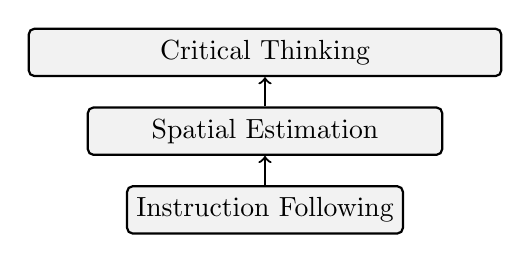
\begin{tikzpicture}[
  box/.style={draw, thick, rounded corners=2pt, minimum width=1cm, minimum height=0.6cm, fill=lightgray!20}
]
  % Critical Thinking
  \node[box, minimum width=6cm] (ct) at (0,2) {Critical Thinking};
  
  % Coord Estimation
  \node[box, minimum width=4.5cm] (ce) at (0,1) {Spatial Estimation};
  
  % Instruction Following
  \node[box, minimum width=3cm] (if) at (0,0) {Instruction Following};
  
  % Connecting lines to show pillar relationship
  \draw[thick, ->] (if.north) -- (ce.south);
  \draw[thick, ->] (ce.north) -- (ct.south);
\end{tikzpicture}
\caption{Capability Hierarchical}
\label{fig:capabilities-hierarchy}
\end{figure}

Penalties include the Invalid Format Penalty and the Invalid Move Penalty. We plan to use the ratio of Invalid Format Penalty as an agent of Instruction Following ability, sort the models by it, compare the result of the same model with reasoning on or off, and see what percentage the reasoning capability adds to the performance. The assumption is that models with better Instruction Following abilities benefit more from the introduction of the reasoning mode. 

We plan to apply the same analysis to Invalid Move Penalty. 

\subsection{Qualitative Samples} 

\textbf{Idea}: 
We plan to do qualitative analysis from the following four angles: Spatial Estimations, Strategy, Critical Thinking, Communication \& Collaboration, and analyze and compare performance across commercial models (Y/N) and reasoning models (Y/N). For GPT-5, we compare across model size (original / mini) as well. 

Here we briefly motivate each of these angles. Concrete examples and analysis will be added later. 

\subsubsection{Spatial Estimation}
From this angle, we check if models can propose valid moving plans. It captures models' Spatial Estimation ability in our grid settings and serves as a foundational pillar of the overall performance. When models are not capable in this regard, they tend to propose invalid moving plans, and attempts to resolve the wrong movements after getting penalties often conduce to cascades of invalid moving plans, therefore quickly exhaust the number of allowed penalties and end up either aborting the game, or attain a low penalty score. 

\subsubsection{Strategy}
In addition to the crude Spatial Estimation, we check how models come up with moving plans. We have observed some smart strategies and their not-so-smart counterparts. In some game plays, one model uses the initial coordinates of the objects to instruct the other model as target locations, thus avoiding penalties of moving objects to cells occupied by the background grids to a large extent; while in some other game plays, models appear to exchange initial coordinates just for the sake of exchanging, without making use of this information. Another example is in some game plays, models choose the most sparse row as the target, and lay objects one by one on it; while in some other game plays, the models unnecessarily chose geometric patterns to lay the objects, such as on the diagonal, disregarding the occupied cells, and run into complexities that they could have dodged. 


\subsubsection{Critical Thinking}
Some models show the ability to critically reason about the moving plan that either itself or the other player proposed. They either refute the plan immediately when it's proposed, or take a sharp brake when they are just about to execute the invalid moving plan. This is, as expected, more frequent in reasoning models compared to non-reasoning models. 
However, on some occasions, we see pseudo-reasoning: a model rejects a correct plan, utters reasoning-like sentences, and proposes another plan that sometimes is correct, sometimes is wrong.


\subsubsection{Communication \& Collaboration}
The above three dimensions positively correlate with the model performance: The better the models are at them, the higher the scores. This dimension, however, is different. Specifically, we observe how models communicate with each other to recover from invalid moves due to target locations being occupied. Some models go at lengths to execute their alternative plans without letting their partner know, they might still have a good score, simply because both player 1 and player 2 adopt the exact same strategy, for example, move the object to one spot next to the original target location. This leads to inflated scores that can be debunked when two models of different default recovery strategies, or one model and one human, play against each other. 

\end{document}